\chapter{Theory and Fundamentals}
\label{chap:theory}

\section{MSME Energy Systems}
Industrial energy consumption is structurally divided into base load and production load. The base load constitutes electricity consumed by baseline systems (e.g., lighting, HVAC, and standby machinery), remaining constant regardless of output. The production load fluctuates directly with manufacturing volume, driven primarily by high-draw inductive motors and thermal elements. In regions with unstable power grids, MSMEs rely heavily on localized Diesel Generators (DG), which carry high operational costs and severe carbon penalties \cite{Zhang2021}. Managing total energy consumption is critical for controlling factory efficiency.

\section{IoT-based Monitoring Architecture}
The Internet of Things (IoT) provides the sensing infrastructure required to digitize physical environments \cite{AlFuqaha2015}. Standard meters track cumulative usage over 30 days. In contrast, edge-device IoT sensors log high-frequency electrical vectors: instantaneous voltage ($V$), running current ($I$), active power ($P = VI\cos\theta$), and frequency distributions. Transmitting this array to cloud-based aggregators enables proactive management, allowing manufacturers to observe sudden power imbalances and inefficient machinery in real time.

\section{Digital Twin Theory}
A Digital Twin is defined as a virtual, dynamic replica of a physical process \cite{Kritzinger2018}. Within the context of energy management, the twin utilizes historical data matrices to mathematically encapsulate the exact behavior of an MSME facility. 

\begin{figure}[h]
    \centering
    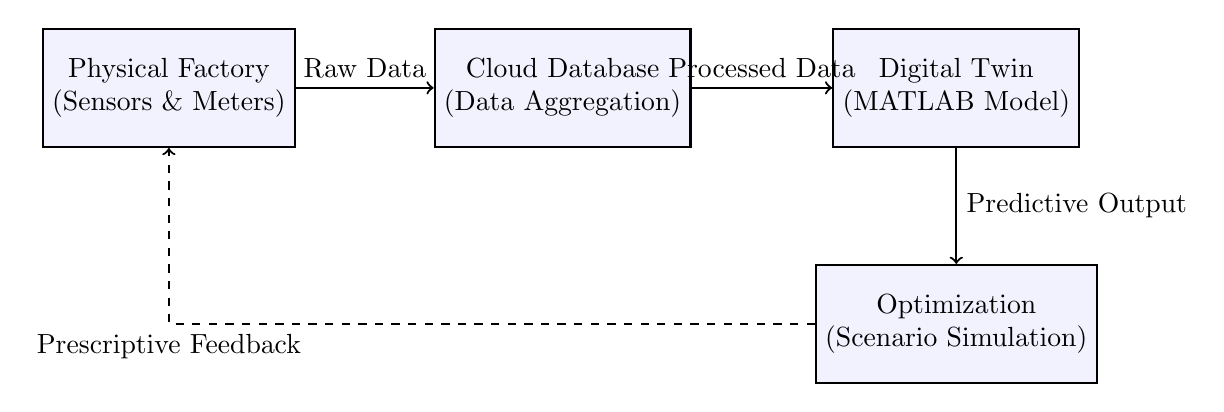
\begin{tikzpicture}[
        box/.style={draw, rectangle, minimum height=1.5cm, minimum width=3cm, align=center, thick, fill=blue!5},
        arrow/.style={->, thick}
    ]
        \node[box] (physical) at (0,0) {Physical Factory\\(Sensors \& Meters)};
        \node[box] (data) at (5,0) {Cloud Database\\(Data Aggregation)};
        \node[box] (twin) at (10,0) {Digital Twin\\(MATLAB Model)};
        \node[box] (opt) at (10,-3) {Optimization\\(Scenario Simulation)};
        
        \draw[arrow] (physical) -- (data) node[midway, above] {Raw Data};
        \draw[arrow] (data) -- (twin) node[midway, above] {Processed Data};
        \draw[arrow] (twin) -- (opt) node[midway, right] {Predictive Output};
        \draw[arrow, dashed] (opt) -| (physical) node[midway, below] {Prescriptive Feedback};
    \end{tikzpicture}
    \caption{Digital Twin Feedback Loop \cite{Tao2019}}
    \label{fig:dt_block}
\end{figure}

As illustrated in Figure \ref{fig:dt_block}, the twin enables simulated testing. Administrators can introduce theoretical changes---such as substituting power sources or isolating production batches---into the model to calculate exact financial outcomes without altering the actual physical plant \cite{Lu2020}.

\section{Machine Learning Prediction Models}
Artificial Intelligence employs optimization methodologies to map input operations to output consumption. Time-series industrial data inherently contains thermodynamic lag and mechanical efficiency loss, which raw linear models fail to capture \cite{Zhang2020}.

\textbf{Linear Regression:} Captures pure proportional scaling but fails at performance saturation boundaries. Equation: $y = w_1x + b$, where $x$ represents production output.

\textbf{Polynomial (Quadratic) Regression:} Handles structural efficiency arcs inherent to heavy machinery, proving significantly more accurate for manufacturing plants. Equation:
$$ \hat{y} = \theta_2 x^2 + \theta_1 x + \theta_0 $$
where $\hat{y}$ is predicted energy, $x$ is production volume, and $\theta_n$ represent trained machine weights capturing baseline usage and performance decay \cite{Tao2018}.

\section{KPI and Sustainability Metrics}
Key Performance Indicators (KPIs) translate electrical physics into business intelligence.
Energy Per Unit (EPU) is the fundamental industrial metric, calculated as:
$$ EPU = \frac{E_{total}}{\text{Production Volume}} $$
Lower EPU indicates superior manufacturing lean-efficiency. Furthermore, Carbon Dioxide emissions estimations (typically scaled at $0.8$ kg CO$_2$ per kWh of diesel energy) provide necessary feedback regarding environmental compliance and footprint monitoring.
